\documentclass[spanish, 11pt]{exam}

%These tell TeX which packages to use.
\usepackage{array,epsfig}
\usepackage{amsmath, textcomp}
\usepackage{amsfonts}
\usepackage{amssymb}
\usepackage{amsxtra}
\usepackage{amsthm}
\usepackage{mathrsfs}
\usepackage{color}
\usepackage{multicol}
\usepackage{verbatim}
\usepackage{svg}

\usepackage[utf8]{inputenc}
\usepackage[spanish]{babel}
\usepackage{eurosym}

\usepackage{graphicx}
\graphicspath{{../img/}}



\printanswers
\nopointsinmargin
\pointformat{}

%Pagination stuff.
%\setlength{\topmargin}{-.3 in}
%\setlength{\oddsidemargin}{0in}
%\setlength{\evensidemargin}{0in}
%\setlength{\textheight}{9.in}
%\setlength{\textwidth}{6.5in}
%\pagestyle{empty}

\renewcommand{\solutiontitle}{\noindent\textbf{Sol:}\enspace}

\newcommand{\samedir}{\mathbin{\!/\mkern-5mu/\!}}

\newcommand{\class}{4º Académicas}
\newcommand{\examdate}{\today}
\newcommand{\examnum}{Funciones}
\newcommand{\tipo}{A}


\newcommand{\timelimit}{50 minutos}



\pagestyle{head}
\firstpageheader{
\includegraphics[width=0.2\columnwidth]{header_left}}{\textbf{Departamento de Matemáticas\linebreak \class}\linebreak \examnum}{
\includegraphics[width=0.1\columnwidth]{header_right}}
\runningheader{\class}{\examnum}{Página \thepage\ of \numpages}
\runningheadrule

\begin{document}

\begin{questions}

\question Calcular el dominio de las siguientes funciones:
\begin{multicols}{2}
\begin{parts}
\part[] $f(x)=\dfrac{x+13}{x^4+x^3-3x^2-3x} $ 
%g = (x+13)/(x**4+x**3-3*x**2-3*x)
%singularities(g, x)
\begin{solution}$\mathbb{R}-\left\{-1, 0, - \sqrt{3}, \sqrt{3}\right\}$ \\
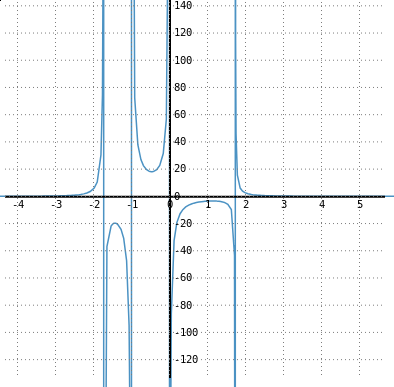
\includegraphics[width=1\columnwidth]{funcion1a}
 \end{solution}

\part[] $f(x)=x^6+x^2-2$ 
\begin{solution} $\mathbb{R}-\emptyset$ \end{solution}

\part[] $f(x)=\dfrac{7x+9}{x^3+8} $ 
%g = (7*x+9)/(x**3+8)
%singularities(g,x)	
\begin{solution} $ \mathbb{R}-\left\{-2, 1 - \sqrt{3} i, 1 + \sqrt{3} i\right\}=\mathbb{R}-\left\{-2\right\}$\\
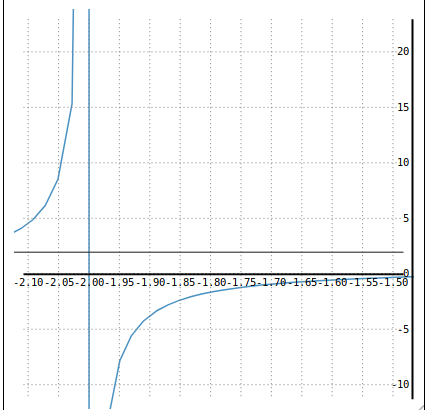
\includegraphics[width=1\columnwidth]{funcion1c}
 \end{solution}
 
%from sympy.solvers.inequalities import reduce_rational_inequalities 
%Complement(S.Reals, reduce_rational_inequalities([[(x-1)/(x) < 0]], x,relational=0))

\part[] $ f(x)=\sqrt{\dfrac{x-1}{x}}$ 
\begin{solution} $\mathbb{R}-\left[0,1\right]=\left(-\infty, 0\right) \cup \left(1, \infty\right)$ \\
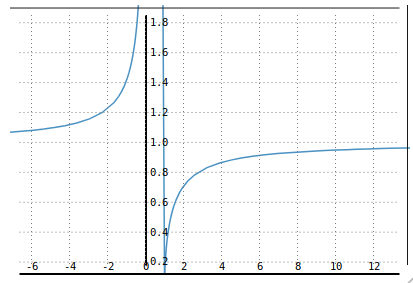
\includegraphics[width=1\columnwidth]{funcion1d}
\end{solution}

\part[] $ f(x)=\sqrt[3]{\dfrac{x-1}{x}} $ 
\begin{solution} $\mathbb{R}-\left\{0\right\}$\\
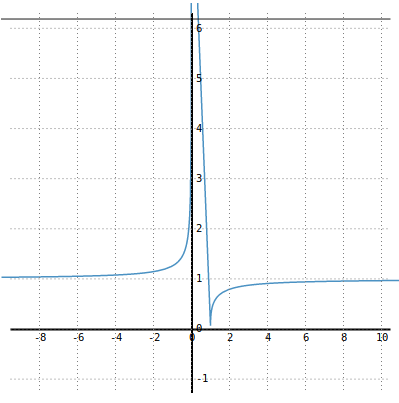
\includegraphics[width=1\columnwidth]{funcion1e}\end{solution}

\part[] $f(x)=\sqrt[4]{\dfrac{x(x+7)}{x^2+5x+6}} $ 
\begin{solution} \end{solution}

\part[] $f(x)=\dfrac{x^3-6x^2+4x+8}{x^3-x^2-9x+9}$ 
% g = (x**3-6*x**2+4*x+8)/(x**3-x**2-9*x+9)
% singularities(g, x)
\begin{solution} $\left\{-3, 1, 3\right\}$ \\

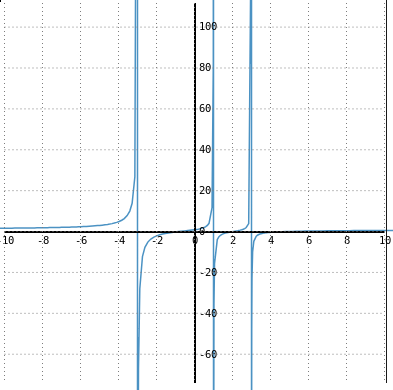
\includegraphics[width=1\columnwidth]{funcion1g}
\end{solution}

\part[] $ f(x)=\dfrac{1}{4x^2-1}$ 
\begin{solution} \end{solution}

\part[] $f(x)=\dfrac{1}{\sqrt[4]{9-x^2}} $ 
\begin{solution} \end{solution}

\part[] $ f(x)=\dfrac{2x+7}{\sqrt[3]{9-x}}$ 
\begin{solution} \end{solution}

\part[] $ f(x)=\dfrac{x^2-5x+6}{\sqrt{x^4-1}}$ 
\begin{solution} \end{solution}

\part[] $f(x)=\sqrt{-2x^2+5x-3} $ 
\begin{solution} \end{solution}

\part[] $f(x)=\dfrac{x^2-3}{x^3-2x^2-x+2} $ 
\begin{solution} \end{solution}

\part[] $ f(x)=\dfrac{5x^3-8}{1+x+x^2}$ 
\begin{solution} \end{solution}

\part[] $ f(x)=\dfrac{x-1}{x^4-7x^2-144}$ 
\begin{solution} \end{solution}

\part[] $f(x)=\dfrac{7x+9}{81x^4-16} $ 
\begin{solution} \end{solution}

\part[] $f(x)=\sqrt[3]{\dfrac{x^6-5x+1}{x^2-4x+4}} $ 
\begin{solution} \end{solution}

\part[] $f(x)=\dfrac{\sqrt{x^2-4x-5}}{x^2+2x+1} $ 
\begin{solution} \end{solution}

\end{parts}
\end{multicols}

\question Dadas las siguientes funciones, dadas por sus gráficas, obtén sus propiedades:

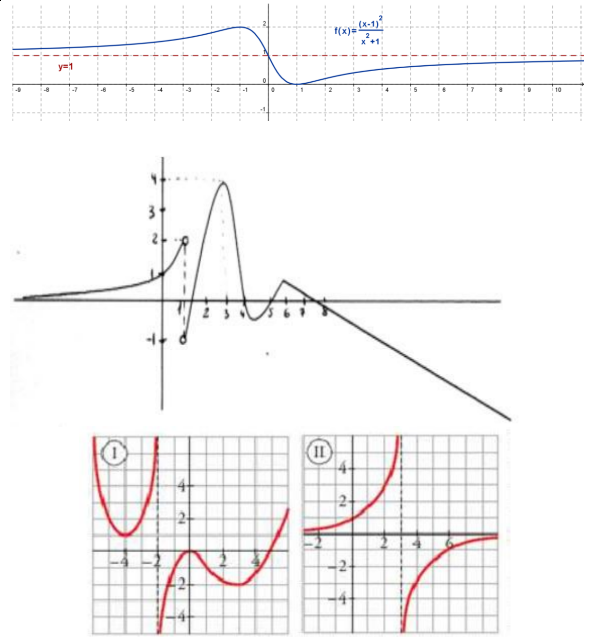
\includegraphics[width=0.61\columnwidth]{funcion2}




\question Representa las siguientes funciones, indicando sus propiedades:
\begin{multicols}{2}
\begin{parts}
\part[] $y=x^2-4x-5$ 
\begin{solution} \end{solution}
\part[] $y=-x^2+4x+5$ 
\begin{solution} \end{solution}
\part[] $y=-x^2-5x+6$ 
\begin{solution} \end{solution}

\part[] $f(x) =
\left\{
	\begin{array}{clc}
		4  & \mbox{si } & x < -2 \\
		-x^2 & \mbox{si } & -2 \leq x < 4 \\
		2x-3 & \mbox{si } & x \geq 4
	\end{array}
\right.$ 
\begin{solution}  \end{solution}

\part[] $f(x) =
\left\{
	\begin{array}{clc}
		2x  & \mbox{si } & x < -3 \\
		x^2-2x-8 & \mbox{si } & -3 \leq x \leq 3 \\
		2x-3 & \mbox{si } & x \geq 3
	\end{array}
\right.$ 
\begin{solution}  \end{solution}

\part[] $f(x) =
\left\{
	\begin{array}{clc}
		x+1  & \mbox{si } & x \leq 0 \\
		x^2-4x+3 & \mbox{si } &  x > 0 
	\end{array}
\right.$ 
\begin{solution}  \end{solution}

\end{parts}
\end{multicols}


\begin{comment}
\question 
\begin{multicols}{3}
\begin{parts}
\part[]  
\begin{solution} \end{solution}
\end{parts}
\end{multicols}
\end{comment}


\end{questions}
\end{document}

